\documentclass{article}
\usepackage{amssymb, amsmath, amsthm}
\usepackage{graphicx}
\usepackage{subcaption}
\title{Homework 1 : Regression}
\author{Elnur Gasanov : 163411}
\parindent=0.0mm


\begin{document}
\maketitle

\textit{Remark}. This doc is the summary of what have been done in the corresponding jupyter notebook file. For technical details, such as numbers of steps, learning rates of algorithms, derivation of the formula of maximum likelihood method, please check the jupyter notebook.

\section{Data Generation}

We use function $f(x) = x^2$ on the interval $[-3, 3)$. Data samples are generated as follows: $t_i = f(x_i) + \varepsilon_i$, where $\varepsilon \in \mathcal{N}(0, 0.2)$. Size of the data set is 200.

Scatter plot of the generated data looks as shown in the figure \ref{GenData}.

\begin{figure*}
	\centering
	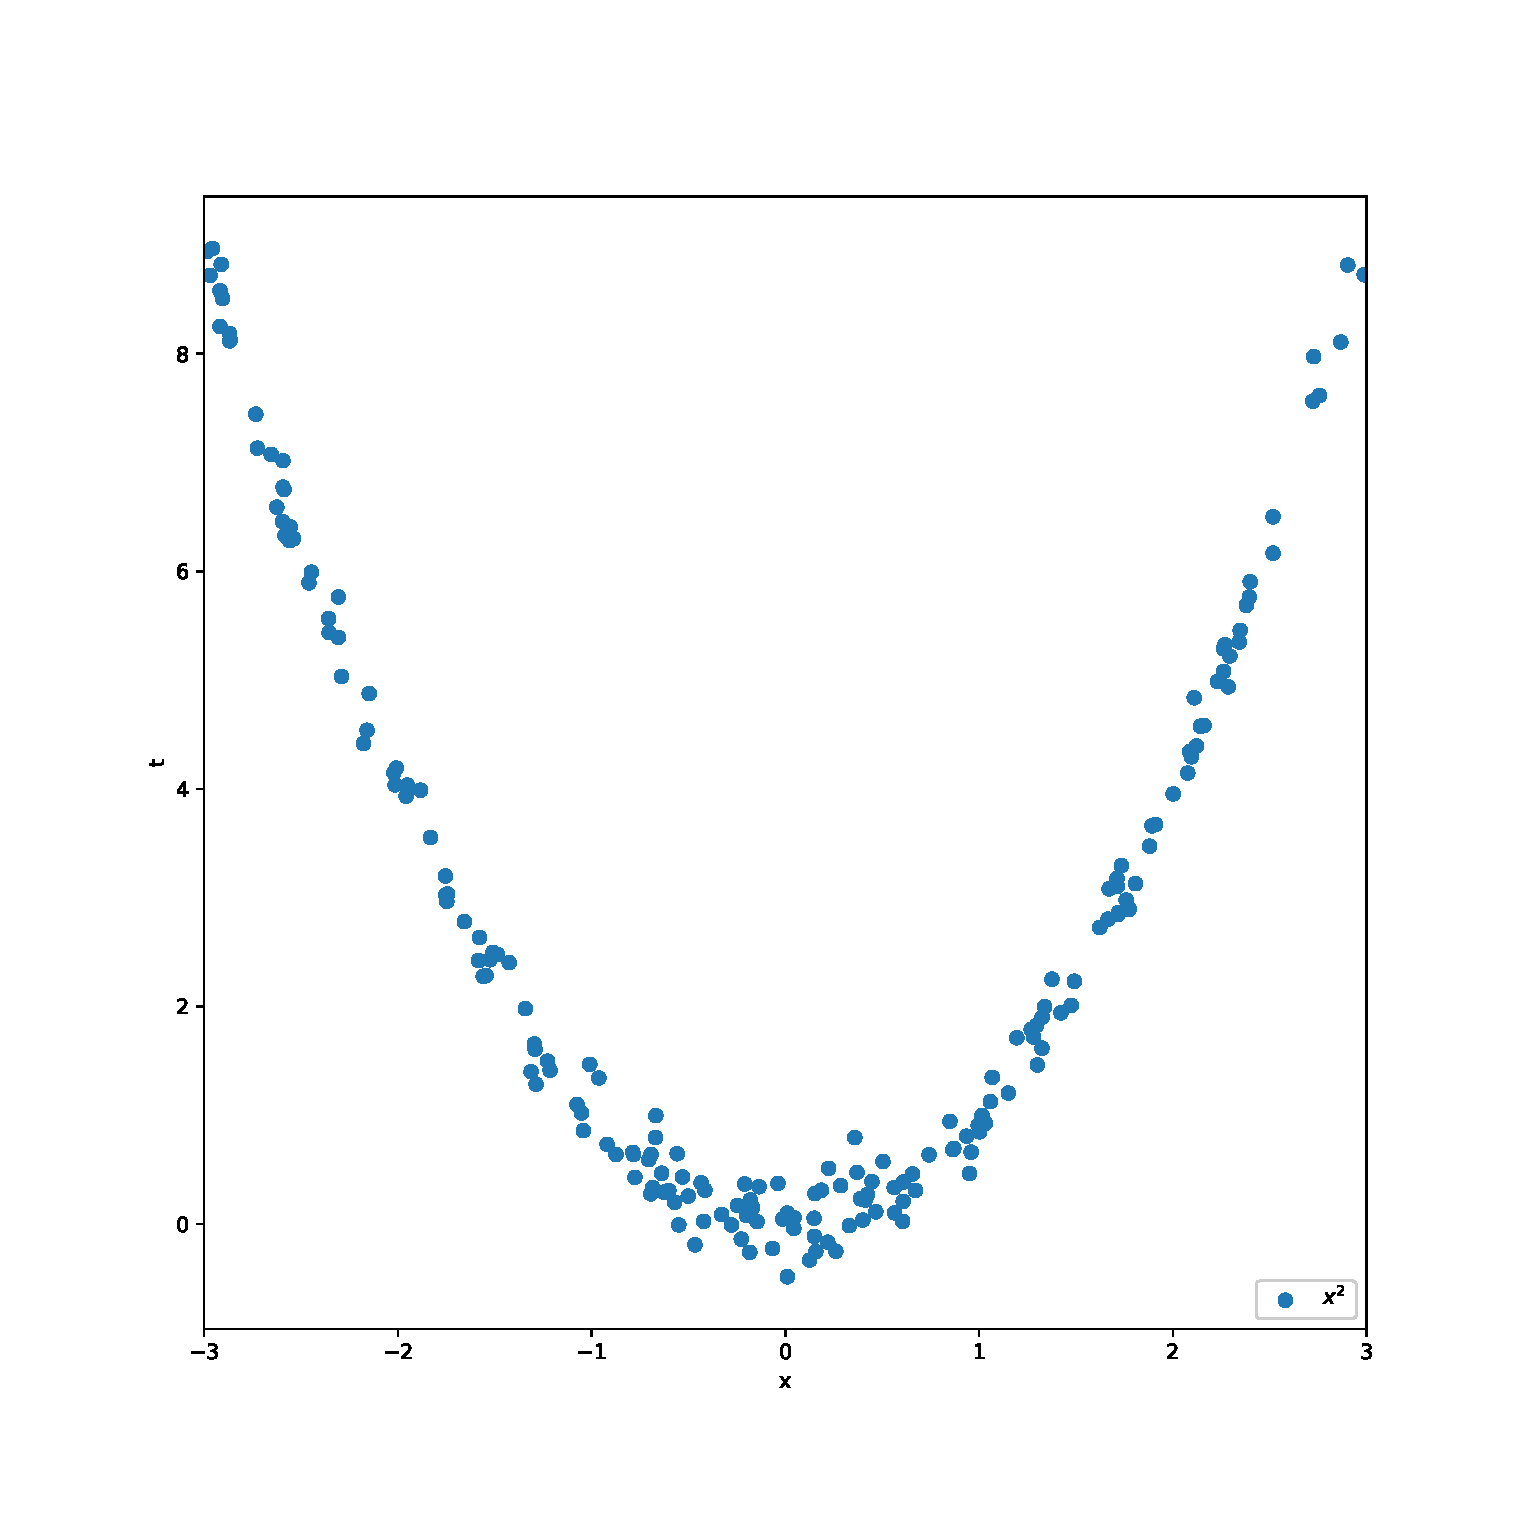
\includegraphics[width = 0.5\linewidth]{raw_data}
	\caption{The generated data}
	\label{GenData}
\end{figure*}

\section{Basis functions, loss function and its gradient}

As basis functions in this task we use $\sin(kx)$ and $\cos(kx)$. We choose 11 basis functions: 
1, $\sin(kx), cos(kx)$, for $k = 1, \dots, 5$.

The loss function on the train data has the following structure:
$$
Q(\{x_i, t_i\}, \overline{w}) = \frac{1}{|Train|}\sum\limits_{i \in Train} (\sum\limits_{j = 1}^{10} w_j \cdot \phi_j(x_i) + w_0 - t_i)^2
$$

Its gradient can be calculated using the formula below:
$$
\nabla Q(\{x_i, t_i\}, \overline{w}) =  \frac{2}{|Train|}\sum\limits_{i \in Train} \left(\sum\limits_{j = 1}^{10} w_j \cdot \phi_j(x_i) + w_0 - t_i \right) \cdot \begin{bmatrix} 1 \\
                                 \phi_1(x_i) \\
                                 \vdots \\
                                 \phi_{10}(x_i)\\
                 \end{bmatrix}
$$
Here $|Train|$ denotes the cardinality of the train data.

\section{Finding optimal $\overline{w} \in \mathbb{R}^{11}$}

Decreasing error function with the increasing number of steps of batch and stochastic gradient descent algorithms is shown in the figure \ref{Error_func} [tasks 1a, 2a].

\begin{figure}[t!]
    \centering
    \begin{subfigure}[b]{0.45\textwidth}
        \centering
        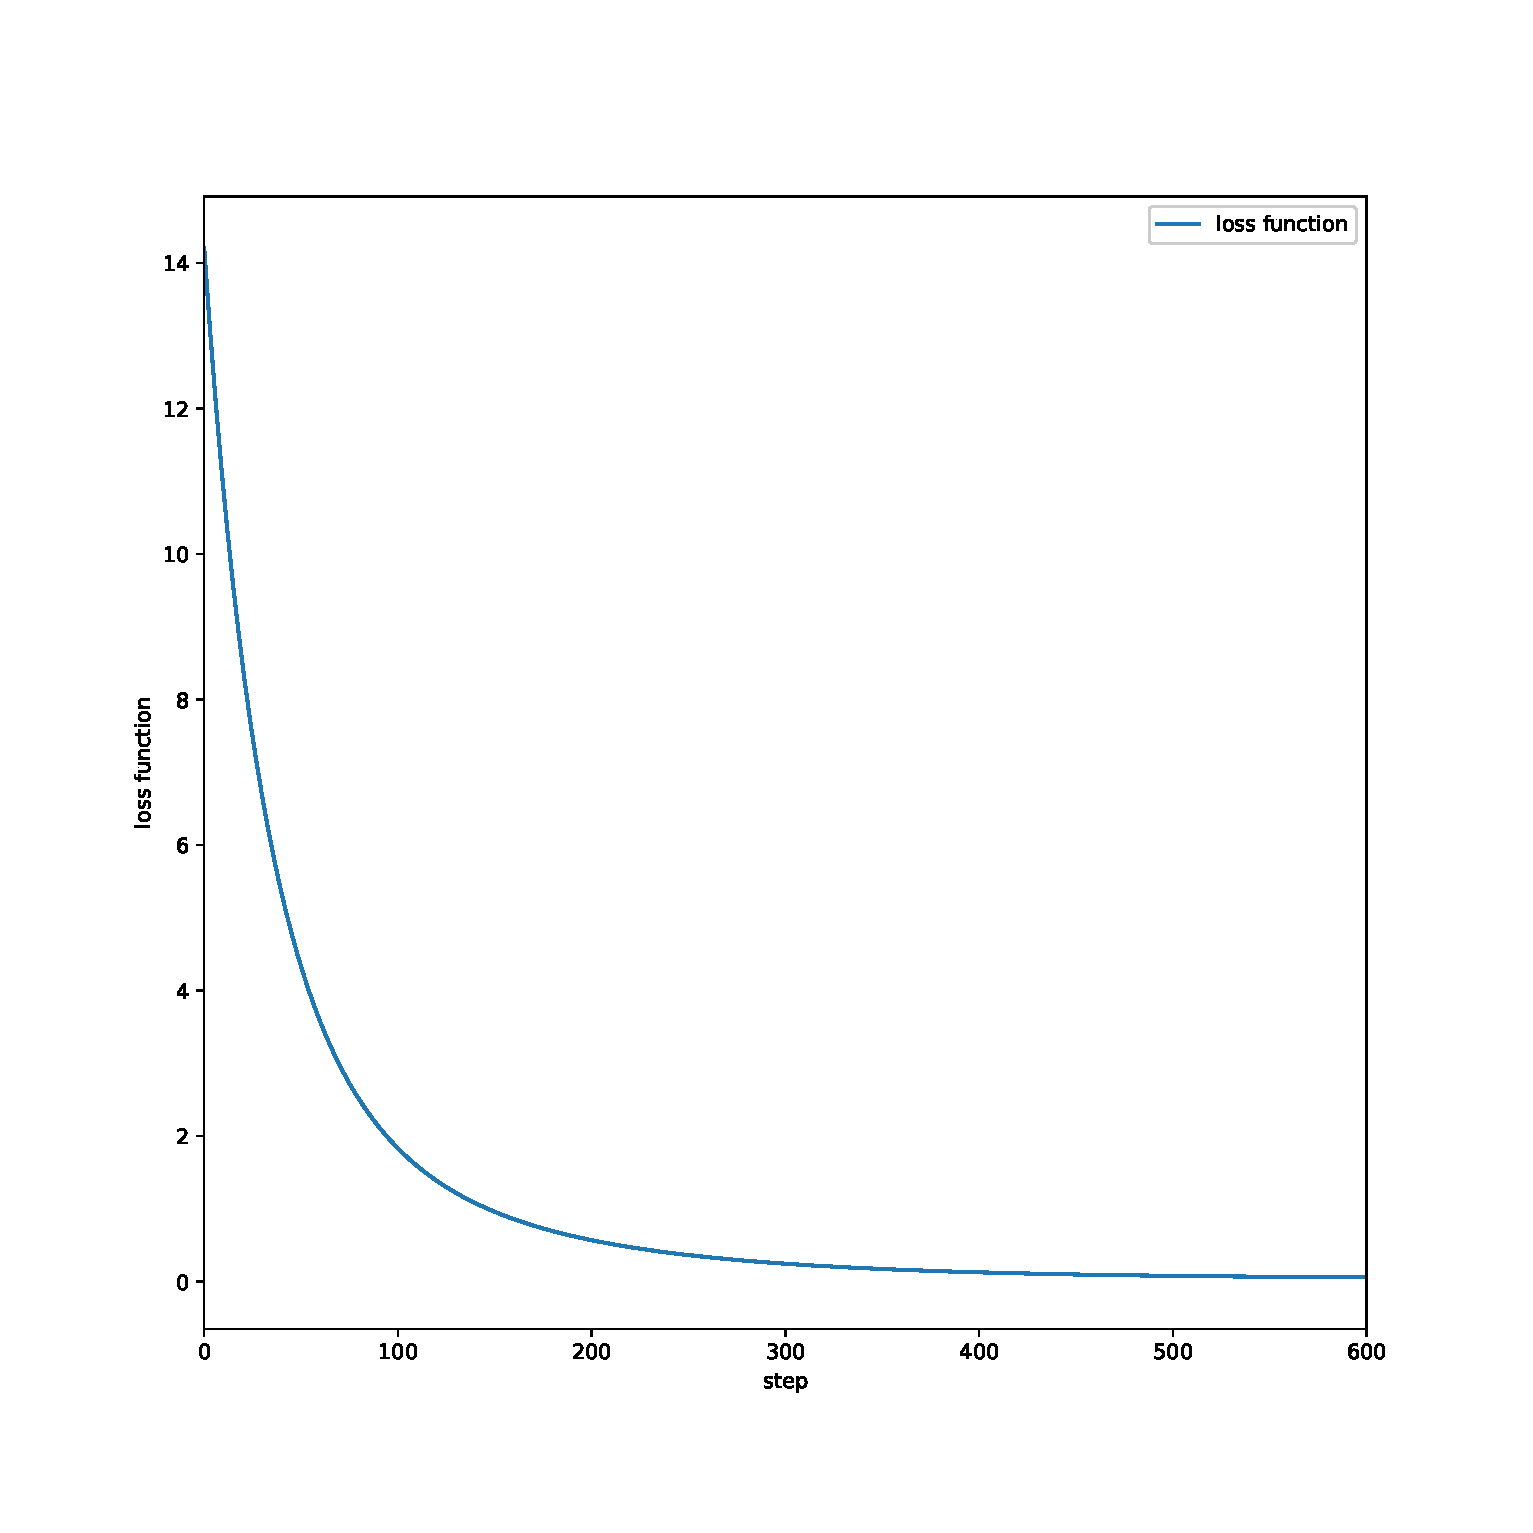
\includegraphics[width = \linewidth]{bgd.eps}
        \caption{batch GD}
    \end{subfigure}
    ~
    \begin{subfigure}[b]{0.45\textwidth}
        \centering
        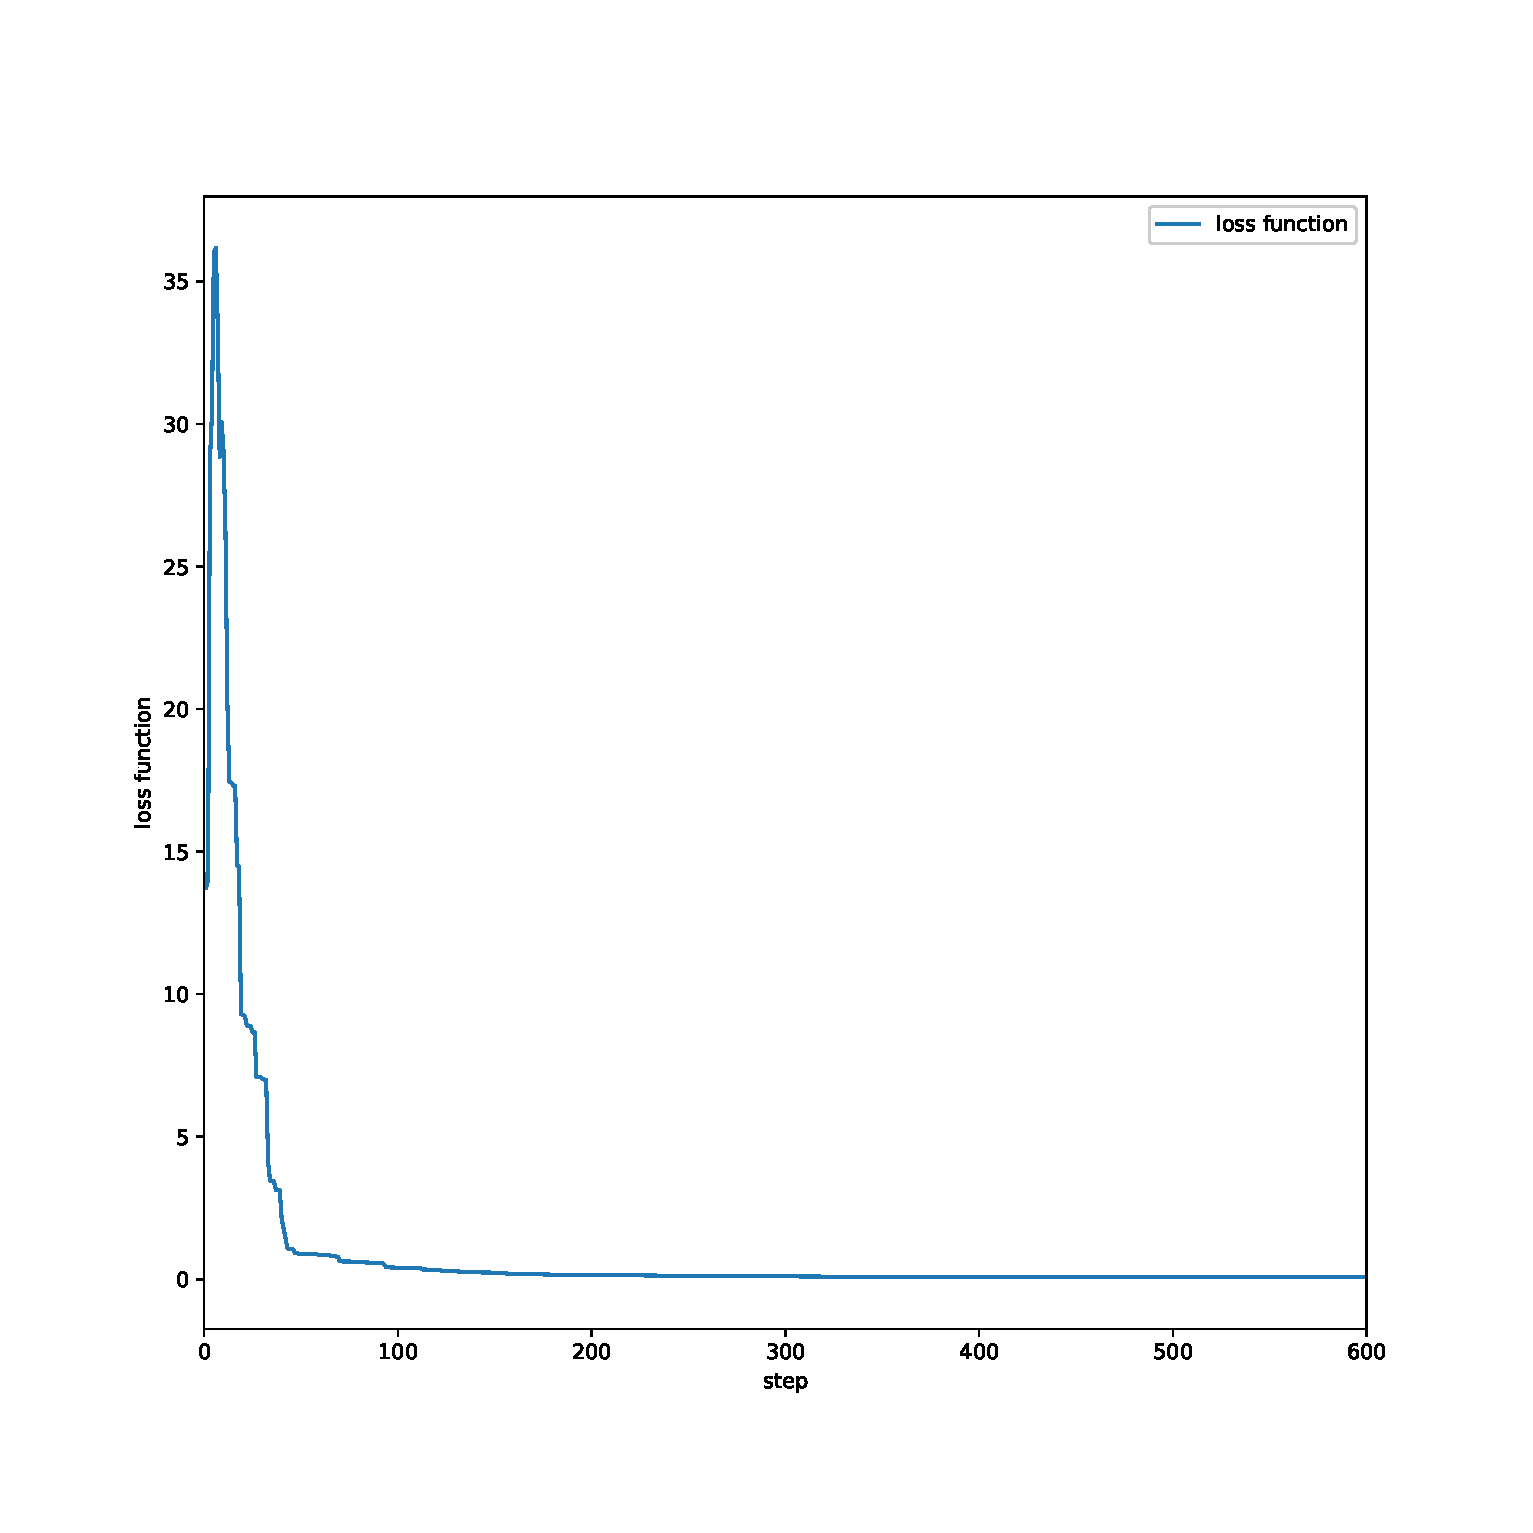
\includegraphics[width = \linewidth]{sgd.eps}
        \caption{stochastic GD}
    \end{subfigure}
    \caption{Decreasing error function with the increasing number of steps}
    \label{Error_func}
\end{figure}

Obtained vectors $w$ are presented in the table \ref{vectors} [tasks 1b, 2b, 3a].

\begin{table*}
\caption{Comparison of the coefficient vectors}
\label{vectors}
\begin{tabular}{|c|l|}
\hline
algorithm & $w$ \\
\hline
batch GD & [3.25, -0.026,  0.025, -0.03,  0.03,
       -0.02, -3.85,  0.84, -0.31,  0.17,
       -0.1] \\
\hline
stochastic GD & [3.28, -0.09,  0.09, -0.0,
       -0.0,  0.0, -3.93,  0.9,
       -0.27,  0.14, -0.13]\\
\hline
maximum likelihood & [3.3,  0.0, 0.0,  0.0,
       -0.0,  0.0, -4.0,  0.96,
       -0.4,  0.24, -0.13] \\
\hline
\end{tabular}
\end{table*}

As can be seen from the table, obtained vectors are quite close: $||w_{lkl}~-~w_{bgd}||_2~=~0.265$, $||w_{lkl}~-~w_{sgd}||_2~=~0.247$ [task 3b].

Learned linear regressions are presented in the figure \ref{predicted_func} [1c, 2c, 3c].

\begin{figure}[t!]
    \centering
    \begin{subfigure}[b]{0.3\textwidth}
        \centering
        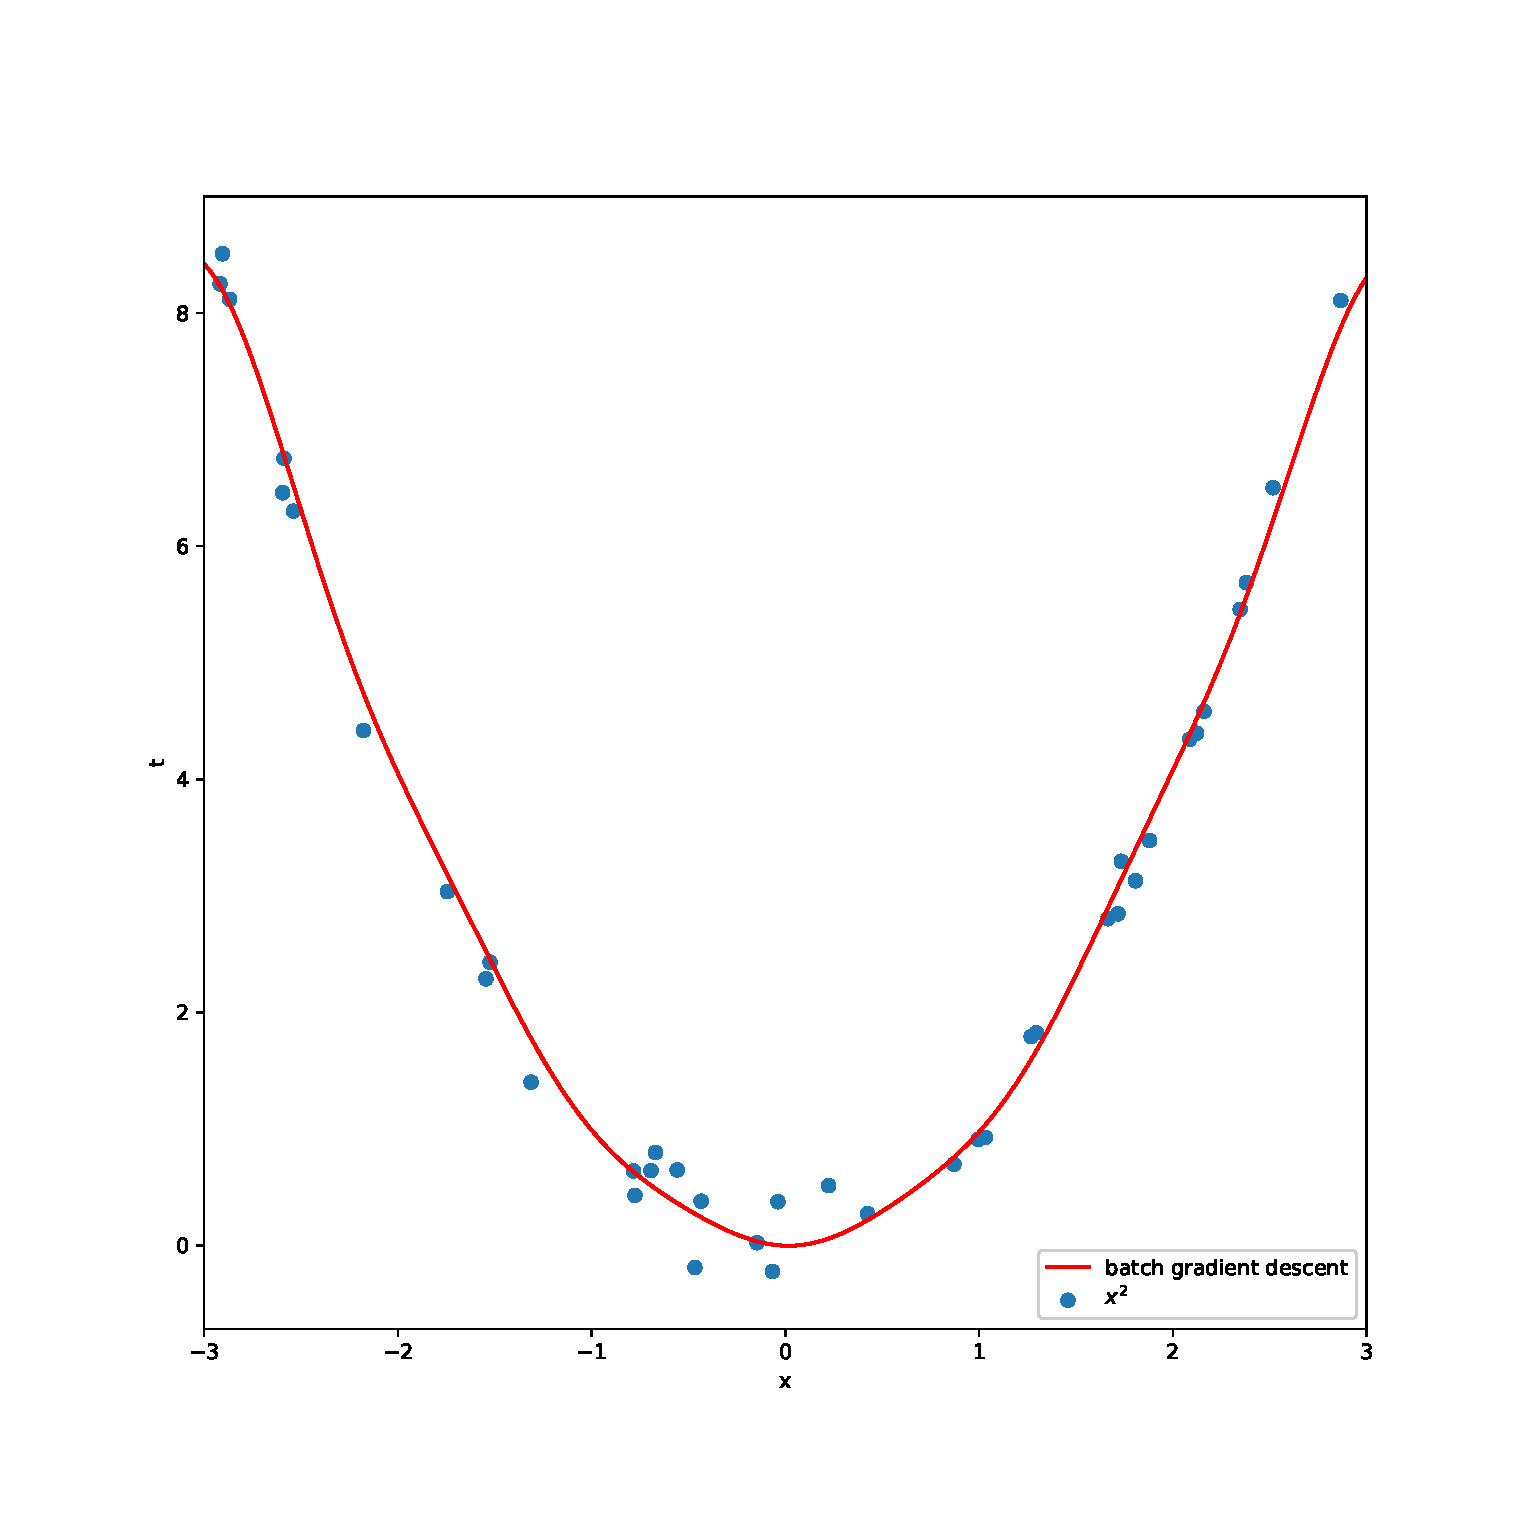
\includegraphics[width = \linewidth]{bgd_final.eps}
        \caption{batch GD}
    \end{subfigure}
    ~
    \begin{subfigure}[b]{0.3\textwidth}
        \centering
        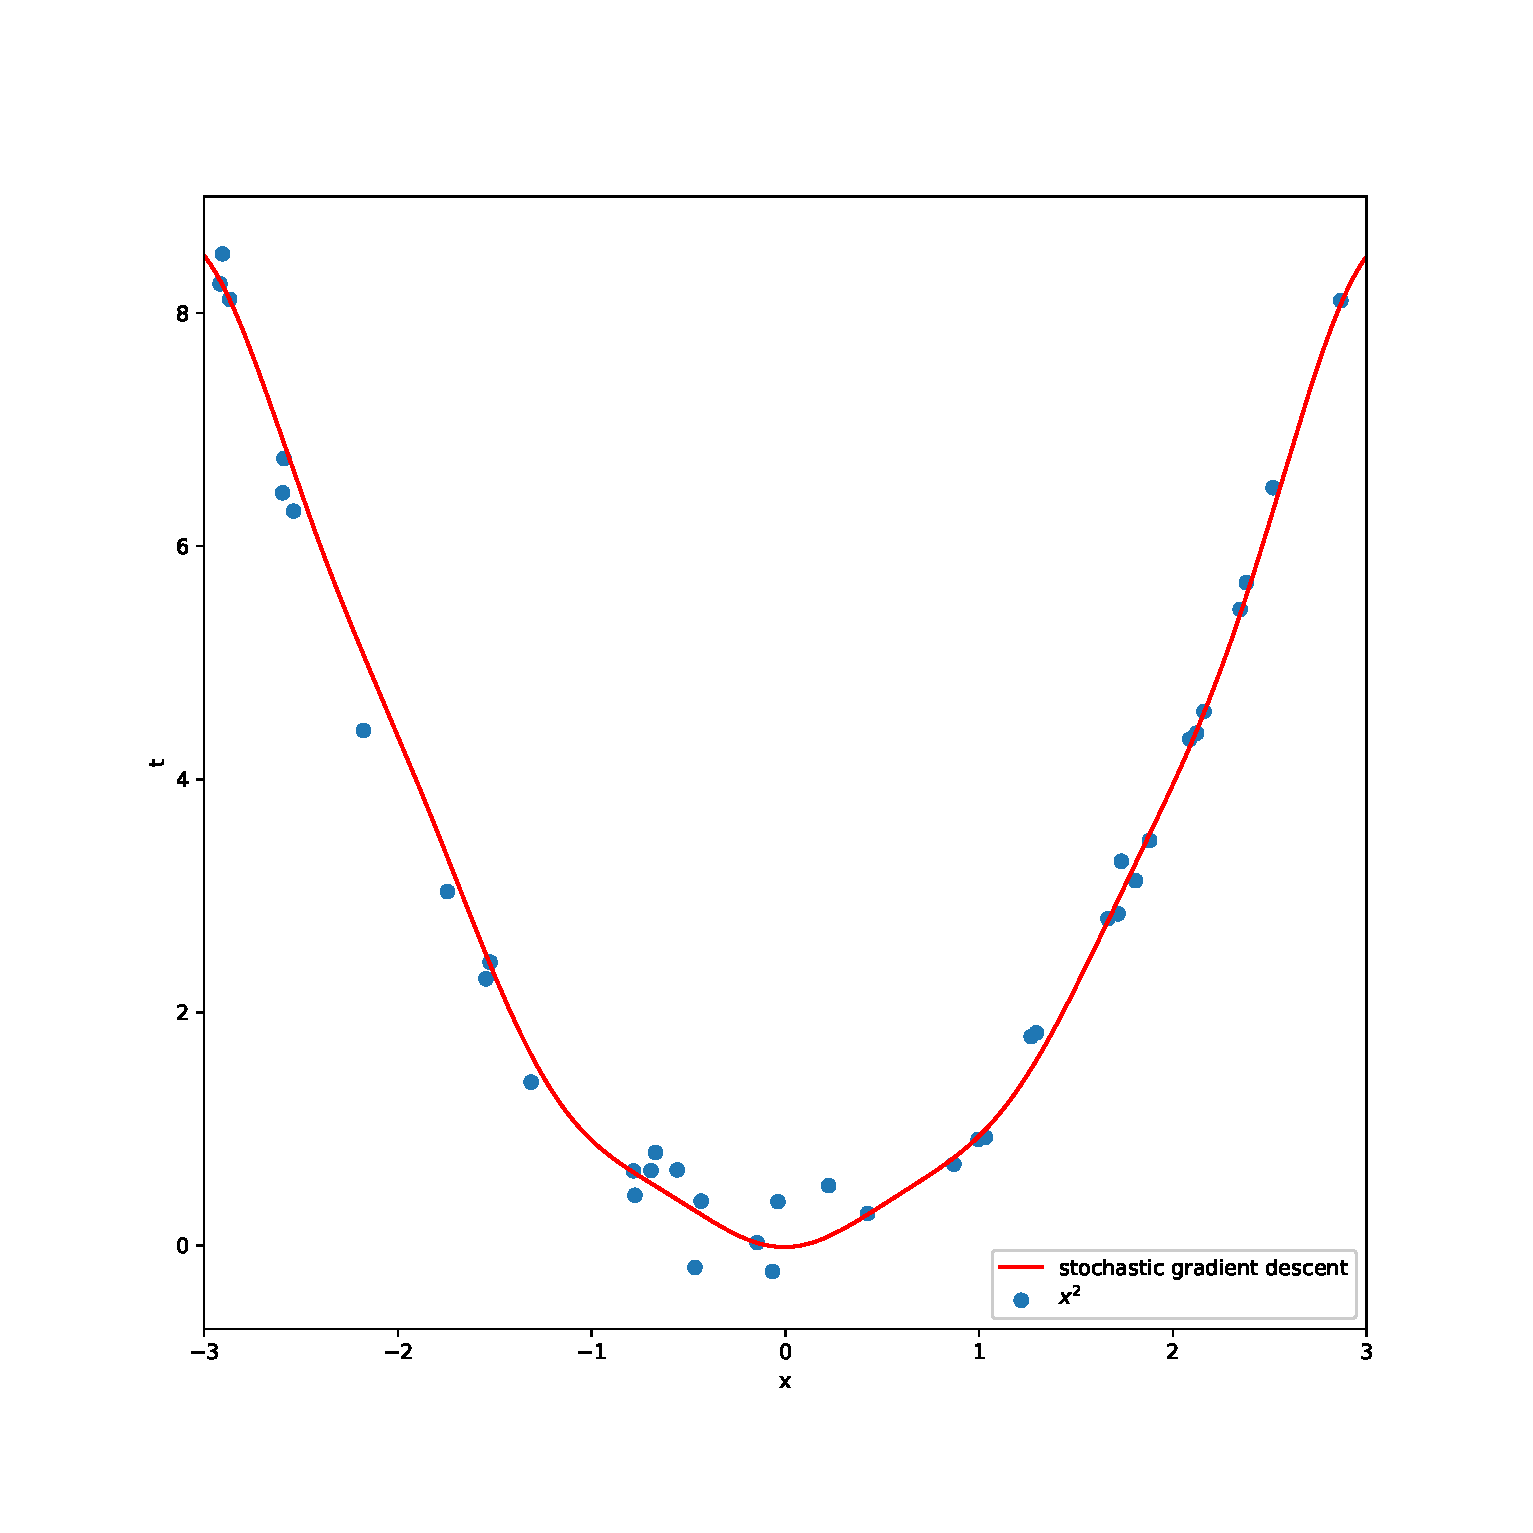
\includegraphics[width = \linewidth]{sgd_final.eps}
        \caption{stochastic GD}
    \end{subfigure}
    ~
    \begin{subfigure}[b]{0.3\textwidth}
        \centering
        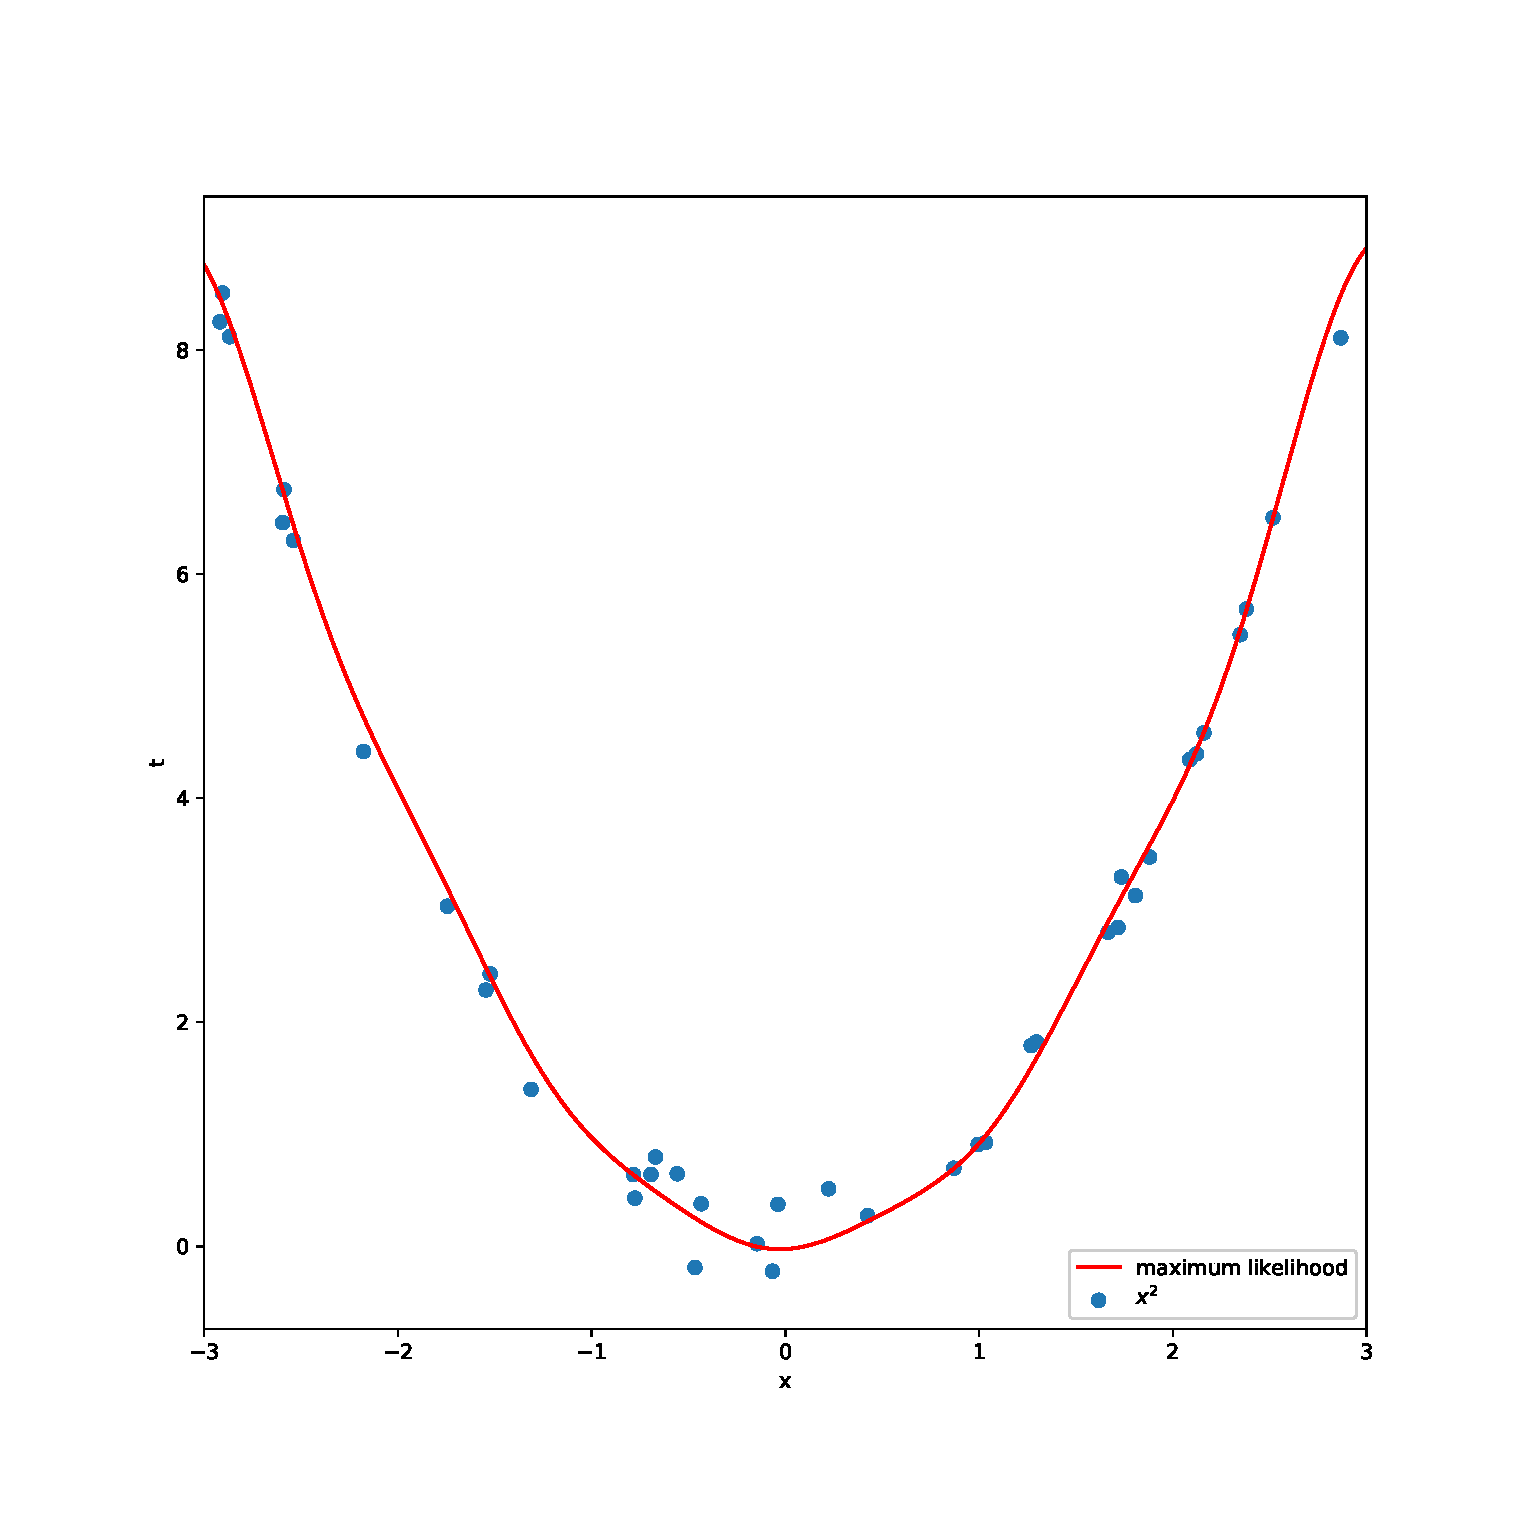
\includegraphics[width = \linewidth]{lkl_final.eps}
        \caption{maximum likelihood}
    \end{subfigure}
    \caption{Predicted $f(x)$ and the test data}
    \label{predicted_func}
\end{figure}

RMSE on the test data are presented in the table \ref{RMSE} [1d, 2d, 3d].

\begin{table*}
\centering
	\caption{Root mean square errors on test data for different algorithms}
	\label{RMSE}
	\begin{tabular}{|c|c|}
	\hline
	algorithm & RMSE \\
	\hline
	batch GD & 0.218 \\
	\hline
	stochastic GD & 0.233 \\
	\hline
	maximum likelihood & 0.203 \\
	\hline
	\end{tabular}
\end{table*}

In this work it appeared to be that the maximum lilelihood approach has the best performance in terms of RMSE on the test data. But, generally speaking, all three approaches solve the same problem of minimizing the squared error of the train data and the maximum likelihood approach solves the problem precisely.

\end{document}